\chapter{Future Work}
\label{c.future}

\section{Eigenspectrum Characterization for Signal Loss}

In Chapter \ref{c.PSmethods}, we discussed how weighting data by an empirical covariance can lead to overfitting of the cosmological signal, resulting in signal loss in a 21\,cm power spectrum. We investigated the relationship between an empirical covariance (namely, its convergence to the true covariance) and the number of independent samples in a data set, and we found, as expected, that convergence rates are fastest when averaging over large numbers of data realizations (Figure \ref{fig:toy_sigloss16}). Additionally, we began to explore the relationship between eigenvector convergence and the shape of an eigenspectrum, finding that steep eigenspectra (with eigenmodes that have eigenvalues that differ greatly from each other) converge the fastest (Figure \ref{fig:toy_sigloss17}).

In this section, we expand our preliminary analysis characterizing covariance eigenspectra and outline future work on this topic. Ideally, we would like to define a metric that relates an eigenspectrum to the amount of potential signal loss it will incur when weighting by it. This would be useful because it would provide a method to estimate, \textit{a priori}, how much signal loss may result given a particular covariance. To define this metric, we must understand how different properties of an eigenspectrum, including its shape and its error bars, affect its convergence. 

We begin with a brief overview in order to develop intuition into how an eigenspectrum affects eigenvector convergence. We recall that a given covariance matrix (which, for our power spectrum analysis is in the frequency domain and describes correlations between frequency channels) can be described by its eigenvalues and eigenvectors. Each eigenvector of a covariance represents a shape, or mode, in the data and has an eigenvalue associated with it. The eigenvalue quantifies how much variance exists along the eigenmode direction, and hence eigenvectors with higher eigenvalues describe shapes with higher amounts of variance. As a reminder, the motivation behind weighting data by a covariance is because the 21\,cm signal is expected to have a frequency structure that differs from foregrounds and other contamination, and we would like to separate out (or up-weight) the cosmological signal with respect to everything else.

As we will soon see, our ability to accurately estimate eigenvalues impacts the convergences of the corresponding eigenvectors to their true forms. The convergences of the eigenvectors, in turn, affects how much signal loss can result when using empirical weighting. As a simple example, suppose we are able to \textit{accurately} estimate \textit{unique} eigenvalues of a covariance (i.e., the eigenspectrum is not flat and has negligible errors). In this situation, there is one well-defined eigenvector associated with each eigenvalue, and our ability to determine them is solely dependent on the number of data realizations as expected. If, however, we are unable to distinguish between individual eigenvalues (i.e., a flat eigenspectrum with repeated values, or an eigenspectrum with large errors so that each eigenvalue is not well-defined and overlaps with others), there is additional room for error in estimating their associated eigenvectors. 

For example, obtaining two degenerate eigenvalues yields some flexibility in determining eigenvectors. Mathematically, we could obtain a solution that is valid --- however, any linear combination of the two eigenvectors we compute are also valid eigenvectors. Given the lack of constraints in this under-determined system, the convergence of the estimated eigenvectors is understandably slowed (and even more data is needed to help with convergence). Another way of describing this effect is that the rate of eigenvector convergence is dependent on the "coupling" or "overlap" between eigenvalues. Ideally, we would like to quickly "de-tangle" estimated eigenvalues (i.e., reduce their errors and avoid a flat eigenspectrum) so that degenerate values do not slow down eigenvector convergence.

To quantify the relationship between an eigenspectrum and eigenvector convergence, we simulate a noise-like EoR signal similarly to Chapter \ref{sec:toymodel_frf}, where we construct a covariance whose true form is a diagonal matrix in the Fourier domain with eigenvalues spanning some range. The Fourier-transform of this covariance is the covariance of the EoR in the frequency domain, or $\textbf{C}_{\rm EoR}$. For different numbers of realizations, we draw random EoR signals that are consistent with $\textbf{C}_{\rm EoR}$ and compute the combined empirical covariance by averaging over the realizations. On the vertical axis of Figure \ref{fig:eigchar_1}, we plot a metric that describes the covariance's empirical eigenvectors $\widehat{\textbf{v}}$ compared to the true eigenvectors $\textbf{v}$, namely Equation \eqref{eq:converge_eig}, or:

\begin{equation}
\label{eq:converge_eig2}
\varepsilon (\widehat{\textbf{v}}) \equiv \sqrt{\sum_{i}^{N_{f}}|\textbf{v}-\widehat{\textbf{v}}|_{i}^2},
\end{equation}
where small $\varepsilon (\widehat{\textbf{v}})$ denotes better convergence, or more agreement with the true eigenvectors.

We run this simulation over a range of realizations and for true covariances whose eigenvalues span a range from one order of magnitude to five (i.e., a relatively flat spectrum to steep). Most importantly, the horizontal axis of Figure \ref{fig:eigchar_1} captures two important properties of an eigenspectrum that we would like to relate to convergence: uncertainty (errors) of the spectrum and relative slope of the spectrum. The reason we choose to look at these two properties is because together they describe how much "overlap" there is between eigenmodes. More overlap (i.e., a flat spectrum and/or large errors) means that there are more possible eigenvector solutions (more linear combinations) given an eigenvalue. This slows down the rate at which the eigenvectors can "de-couple" and approach their true forms. 

In practice, the eigenvalue errors in our simulation come from the distribution of empirical eigenvalues obtained from running $N$ total simulations, where $N$ is large. The quantity we then form for every $i^{th}$ eigenmode (except the smallest one, when ordered from largest to smallest) is a fractional error (FE):

\begin{equation}
FE = \frac{\sigma_{i} + \sigma_{i+1}}{2(\lambda_{i} - \lambda_{i+1})},
\end{equation}
where $\sigma$ are eigenvalue errors and $\lambda$ are eigenvalues. This quantity thus captures both how much overlap there is between eigenvalues (the numerator, or average of two adjacent errors) and how steep the spectrum is (the denominator). 

\begin{figure}
    \centering
	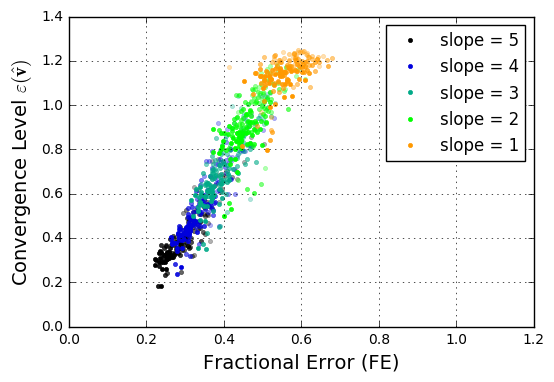
\includegraphics[width=0.63\textwidth]{plots/eigchar_1.png}    
	\caption{The convergence level (y-axis, where convergence is better when eigenvector differences are small), as defined by Equation \eqref{eq:converge_eig2}, of empirically estimated eigenvectors compared to a fractional error metric of the eigenspectrum (x-axis) which takes into account both how well-defined and how steep the spectrum is. The different colors denote the number of orders of magnitude that the true eigenspectrum spans. It appears that the defined fractional error quantity is closely related to eigenvector convergence, with smaller errors and steeper spectrum slopes showing better convergence.}
    \label{fig:eigchar_1}
\end{figure}

\begin{figure}
    \centering
	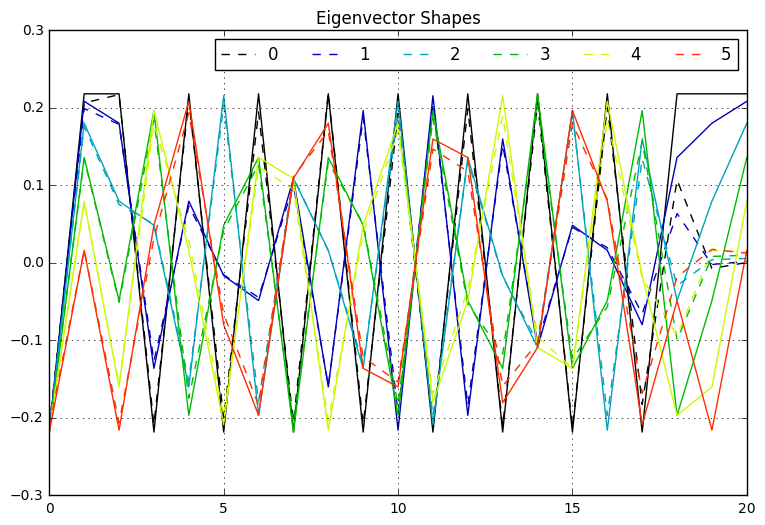
\includegraphics[width=0.63\textwidth]{plots/eigchar_3.png}    
	\caption{Eigenvector shapes for a few of the first modes (different colors) for the simulation corresponding to $N_{real}=100$ in Figure \ref{fig:eigchar_2}. The empirical eigenvectors (dashed) are in general converged to their true forms (solid), implying minimal signal loss. However, we see what seems like perceived signal loss in Figure \ref{fig:eigchar_2}, which is later determined to be a deviation caused by an unrelated issue.}
    \label{fig:eigchar_3}
\end{figure}

\begin{figure}
    \centering
	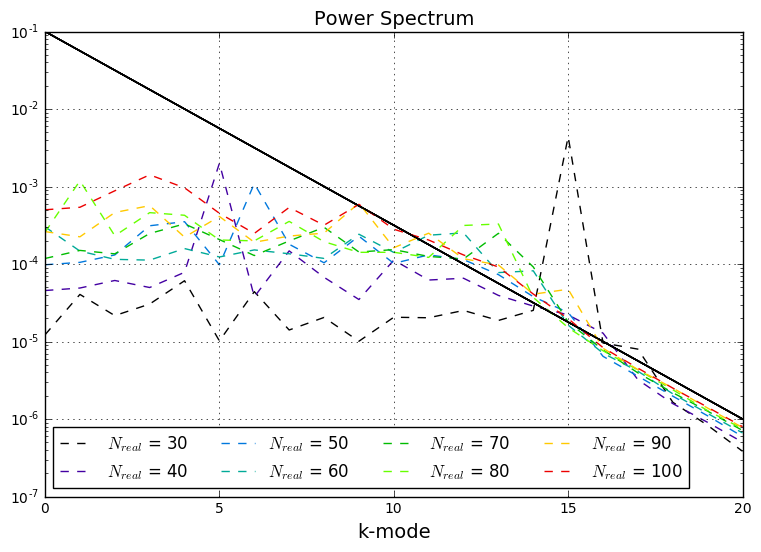
\includegraphics[width=0.63\textwidth]{plots/eigchar_2.png}    
	\caption{Resulting power spectra for different numbers of realizations (dashed colors) compared to the true power spectrum (solid black), which spans five orders of magnitude. Although increasing the number of realizations decreases loss as expected, there is still perceived signal loss at high-amplitude $k$-modes (which is later determined to be a deviation caused by an unrelated issue).}
    \label{fig:eigchar_2}
\end{figure}

From Figure \ref{fig:eigchar_1}, we see that the fractional error quantity we defined is closely related to eigenvector convergence, with eigenspectra with smaller errors converging fastest. Looking at the different colors, we also see that eigenspectra with steeper slopes converge fastest, which is in alignment with our discussion above. We have therefore showed how eigenvector convergence depends on properties of an eigenspectrum, and our next step is to relate convergence to signal loss. 

Up until now, we have implied that a converged covariance (and more specifically, converged eigenvectors) is synonymous with minimal/no loss (i.e., what we would like to achieve). This would mean that given an eigenspectrum, all we would have to do is calculate the fractional error metric as defined above in order to determine how well-converged it is, and therefore how much signal loss there is. As an example, we can zoom in to look at the empirical eigenvectors for the simulation with the steepest slope (slope of five orders of magnitude, or the black points in Figure \ref{fig:eigchar_1}). Figure \ref{fig:eigchar_3} compares five of these eigenvectors (dashed) with their true shapes (solid), and we generally see good agreement between the two.

Figure \ref{fig:eigchar_3} implies that the eigenvectors in our simulation have nearly converged. Hence, we expect minimal signal loss in the resulting power spectra. It is peculiar then, that our power spectrum result in Figure \ref{fig:eigchar_2} displays what looks like signal loss at the highest amplitude $k$-modes. A naive interpretation of this figure may be that empirical inverse covariance weighting has led to loss; however, since we have seen that the eigenvectors have in fact converged, this conclusion would be incorrect.

\begin{figure}
    \centering
	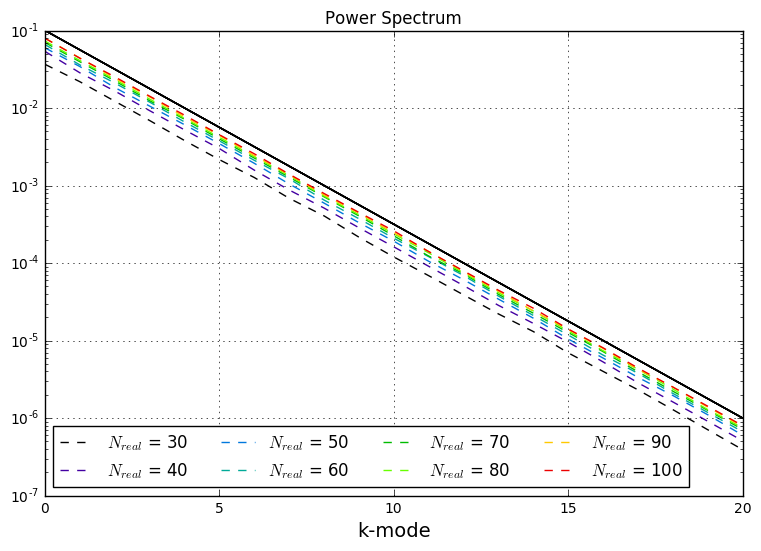
\includegraphics[width=0.63\textwidth]{plots/eigchar_4.png}    
	\caption{Resulting power spectra for different numbers of realizations (dashed colors) compared to the true power spectrum (solid black), which spans five orders of magnitude. This plot differs from Figure \ref{fig:eigchar_2} only in window function shapes; here our window functions are tailored to estimate power spectrum modes independently from each other. We find that by de-tangling window function modes, we avoid power spectrum deviations such as in Figure \ref{fig:eigchar_2} where information from high $k$-modes are dragging down low $k$-modes.}
    \label{fig:eigchar_4}
\end{figure}

Analyzed in isolation, Figure \ref{fig:eigchar_2} is misleading. Increasing the number of realizations (different colors) decreases the perceived loss as expected, but the discrepancy between the estimated and true power spectrum does not actually stem from empirical inverse covariance weighting, which has been the focus of much of this thesis. Instead, deeper investigations reveal that the origin of the deviation can be attributed to the shapes of the window functions that are used in power spectrum estimation. 

Let's explore this in a bit more detail. Recall that the window function relates our estimated power spectrum $\widehat{\textbf{P}}$ to the true power spectrum $\textbf{P}$ (Chapter \ref{sec:QE}):

\begin{equation}
\widehat{\textbf{P}} = \textbf{W}\textbf{P}.
\end{equation}
Window functions describe how different $k$-modes are related to each other --- peaky window functions draw power spectrum information from independent $k$-modes, while long-tailed window functions mean that power spectrum modes draw information from multiple modes. Hence, window functions have the potential to entangle modes in a similar way that flat (or large-error) eigenspectra can. Indeed in our previous simulation we chose a normalization matrix such that our window functions for the low-value $k$-modes were heavily influenced by information from high-value $k$-modes, essentially dragging down the power spectrum at low $k$'s.

As a useful check, we can force our window functions to be $\textbf{W} = \textbf{I}$, or the identity matrix, so that each $k$-mode is estimated independently from each other. In practice, this is done by choosing our normalization matrix $\textbf{M}$, where $\textbf{W} = \textbf{M}\textbf{G}$ (Chapter \ref{sec:MitBias}), in such a way so that $\textbf{W} = \textbf{I}$. In doing so, our resulting power spectrum estimates deviate much less from the true power spectrum (Figure \ref{fig:eigchar_4}). From this analysis, it is clear that power spectrum deviations can disguise themselves as signal loss when in fact window functions are playing an unexpected role. In the future, it will be necessary to balance the advantages of wide window functions (which are typically chosen to minimize vertical power spectrum errors) with the potential power spectrum deviation that can result.

In this section we have seen how the convergence of empirical eigenvectors is related to both the shape of an eigenspectrum and how well defined the spectrum is (which is dependent on number of realizations). We have also shown how power spectrum estimates are affected by the choice of window functions used in power spectrum estimation. In summary, we conclude that steeper eigenspectra, larger eigenvalue errors, and fewer data realizations all increase signal loss in combination with empirical inverse covariance weighting. Analyzing the convergences of eigenvectors is in general a good indicator of potential loss; however, it is not a complete explanation for power spectrum deviations. Instead, window functions can take an accurate, non-lossy result --- and modify it in a way that mimics loss in a final estimate. 

Future work is needed in order to tie these individual relationships together to form one easily computable metric that can be used to map eigenspectrum and window function properties to a specific amount of power spectrum deviation. The goal for this characterization is to intimately understand the interplay between all the effects in order to be able to bridge data properties into a theoretical estimate for loss/deviation. For example, one hopes to be able to look at a HERA eigenspectrum that's computed solely from data, place some error bars on the spectrum based on a theoretical estimate of noise and how many data samples are used, and then characterize the spectrum and use this information to inform decisions about power spectrum weighting. Developing an intuition and quantitative approach for estimating signal loss associated with a particular covariance and eigenspectrum will be extremely powerful for assessing power spectrum results and will save computational time by providing a way to estimate loss without having to perform expensive simulations that quantify loss after-the-fact. 

As the 21\,cm community moves towards more rigorous analysis techniques and EoR sensitivities, the work in this section, as well as future work deepening our understanding of empirical covariances and signal loss, complement a general desire for new techniques that help shape and motivate power spectrum analysis choices.

\section{HERA}

The full HERA array is nearing its completion in construction, and preliminary HERA analyses are ongoing. While this thesis focuses on power spectrum methods as applied to PAPER, the lessons we have learned are already influencing HERA analysis. More specifically, we showed how aggressive fringe-rate filtering of PAPER data leads to lossy, inaccurate power spectra; consequently HERA's initial power spectrum results will use data that is not fringe-rate filtered. With PAPER we illustrated how empirical inverse covariance weighting is coupled with substantial loss and how regularization of those covariances does not seem to carry a significant advantage over uniform weighting; hence HERA analysis is currently focused on forming unweighted power spectra.

Similarly, investigations of bootstrapping and error estimation in PAPER have influenced a HERA power spectrum pipeline that now computes power spectrum errors in a variety of ways, including via bootstrapping, propagation, histogramming, noise realizations, and simulations. Pure noise simulations, which we first introduced as a way to help verify PAPER's sensitivity, are now routinely processed as part of HERA's validation. PAPER discoveries regarding the effect of correlated data samples on error estimation have inspired deeper investigations into other subtleties surrounding correlated noise and bootstrapping. And discussions of systematics and the implementation of jackknife tests for PAPER have contributed in setting a new standard for HERA in terms of establishing useful, routine tests.

In general, the work in this thesis has helped to raise the bar for thorough HERA analysis. It has inspired more detailed documentation, more well-defined tests, more eyes on data, and a more urgent desire for nuanced understandings, cross-checks, and validation. With this strong foundation, HERA is positioned well to produce robust, believable results and tackle challenges that lay ahead. 



